\section{Theorie}
Kryptografie befasst sich mit der Verschlüsselung von Daten, sodass nur Sender und Empfänger die Nachricht lesen können. Die Sicherheit basiert entweder auf komplexen Algorithmen oder praktischen Hindernissen wie der Faktorisierung großer Zahlen. Klassische Verfahren sind jedoch nie absolut sicher, da Schlüssel geknackt werden können. Mithilfe der Quantenphysik lässt sich dieses Problem lösen, indem ein zufälliger Schlüssel generiert wird, der nur Sender und Empfänger bekannt ist. Abhörversuche werden dabei grundsätzlich erkannt.
Der Analogieversuch wird mit dem sgn. BB84 Protokoll durchgeführt %\cite{bennett1984quantum}.
\subsection{One-Time Pad}
\label{sec:Blabla}
Das One-Time Pad ist ein Schlüsselverfahren mit einem zufällig generierten schlüssel aus bits, welcher auf die zu verschlüsselnde Nachricht addiert werden soll.
Hierbei sind die gelten die Regeln
\begin{align*}
    0 &+ 0 =0\\
    1 &+0 =1\\
    0&+1 =1\\
    1&+1=0\; .
\end{align*}
Falls ein Abhörversuch stattfindet, kann die Nachricht also nur entschlüsselt werden, wenn der zufällig gewählte Schlüssel bekannt ist.
Die Voraussetzungen für die Sicherheit des Verfahrens sind 
\begin{enumerate}
    \item Die Länge des Schlüssels entspricht der Nachrichten Länge,
    \item Einmalige Verwendung eines Schlüssels,
    \item Komplett zufällige Wahl des Schlüssels,
    \item Schlüssel darf nur dem Sender und Empfänger bekannt sein.
\end{enumerate}

Punkt 3 und 4 sind im klassischen Sinn schwierig umzusetzen, da klassische Zufallszahlen bei genauer Betrachtung nur pseudozufällig als Ergebnis eines Algorithmus sind und die Übermittlung eines Schlüssels prinzipiell auch Abgefangen werden könnte.
Diese Probleme können durch die Quantenmechanik gelöst werden.

\subsection{Erstellung eines Schlüssels}
Für die Erstellung eines Schlüssels ist es nötig vorab die Darstellung der Bits zu diskutieren. Hierzu wird der Sender, der im Folgenden Alice genannt wird genutzt.
ALice möchte eine verschlüsselte Nachricht an den Empfänger Bob senden. Hierzu müssen die Bits übertragen werden. Grundsätzlich beinhaltet die Wahl des Bits nur ob das gesendete Photon horizontal ("0") oder vertikal 
polarisiert ("1") polarisiert ist. 
Die Polarisationsrichtung wird über die Verwendung einer $\lambda/2$-Platte realisiert. 
Eine $\lambda/2$-Platte ist ein optisches Element aus einem doppelbrechenden Material, das dazu dient, die Polarisationsrichtung von Licht gezielt zu drehen. Die Funktion basiert auf der Eigenschaft der Doppelbrechung, bei der Licht in zwei Komponenten, die schnelle Achse und die langsame Achse, aufgeteilt wird, die unterschiedlich schnell durch das Material laufen. Licht, das entlang der schnellen Achse polarisiert ist, bewegt sich schneller, während Licht, das entlang der langsamen Achse polarisiert ist, verlangsamt wird.
Der Unterschied in der Geschwindigkeit führt zu einer Phasenverschiebung zwischen den beiden Lichtkomponenten. Für eine $\lambda/2$-Platte beträgt die Phasenverschiebung genau eine halbe Wellenlänge, also $180^\circ$. Wenn linear polarisiertes Licht in die $\lambda/2$-Platte eintritt, wird die Polarisationsebene um einen Winkel gedreht, der doppelt so groß ist wie der Drehwinkel der Platte relativ zur ursprünglichen Polarisationsrichtung.
\begin{figure}[H]
	\centering
	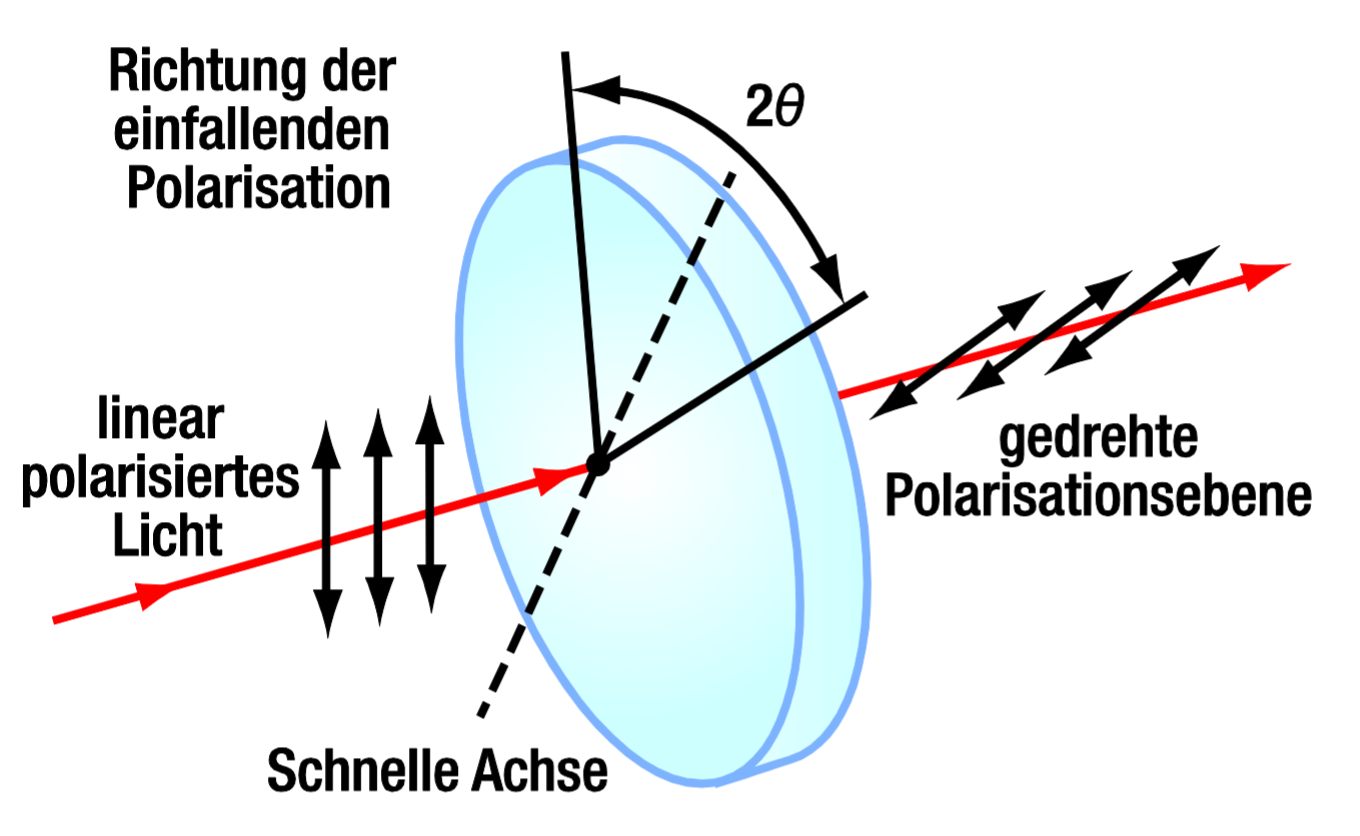
\includegraphics[width=0.75\textwidth]{content/grafik/lambdahalbe.png}
	\caption{Schematische Darstellung der Funktionsweise eines $\lambda /2$-Plättchen. \cite{krypt}}
	\label{fig:lambda}
\end{figure}
Eine schematische Darstellung der Funktionsweise einer $\lambda/2$-Platte ist in \autoref{fig:lambda} dargestellt.
Bob kann die Polarisationsrichtung unterscheiden, indem vor den verwendeten Detektoren (siehe \autoref{sec:Aufbau}) einen polarisierenden Strahlteiler verwendet, welcher in \autoref{fig:Strahlteiler} gezeigt ist.

\begin{figure}[H]
	\centering
	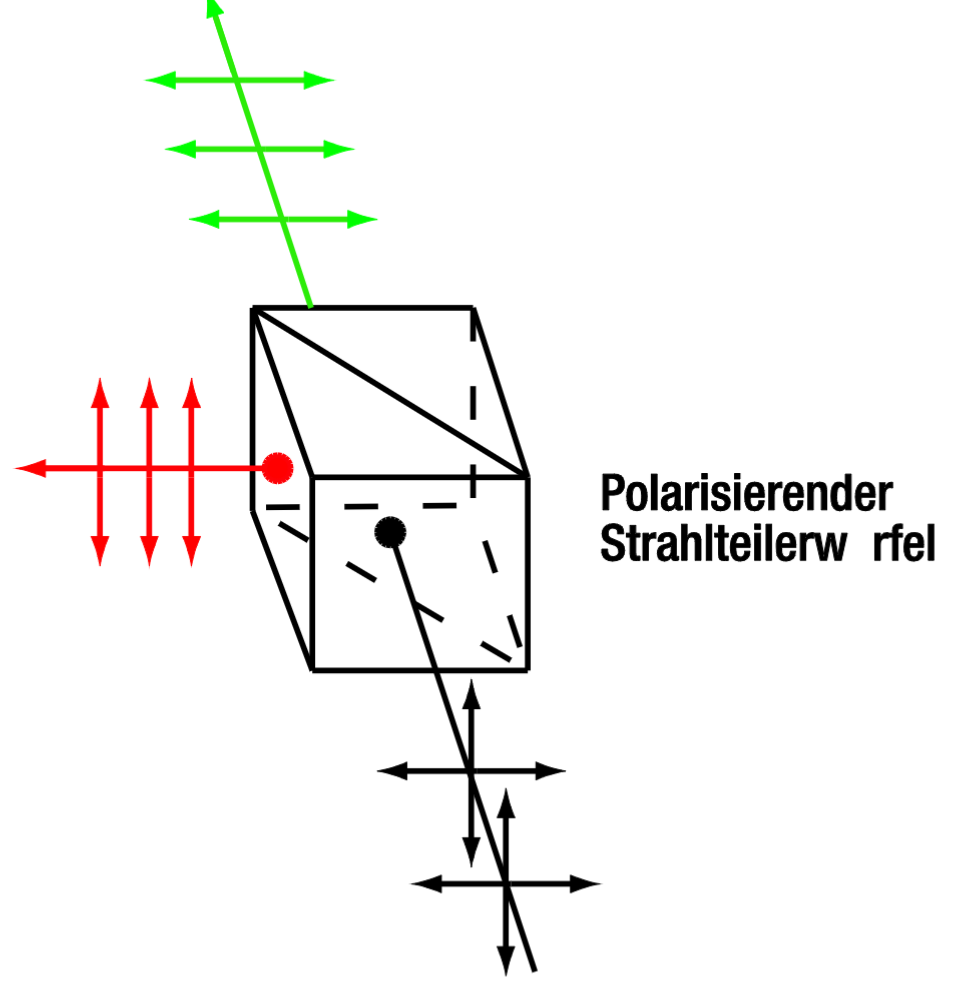
\includegraphics[width=0.75\textwidth]{content/grafik/Strahlteiler.png}
	\caption{Darstellung eines polarisierenden Strahlteilers. \cite{krypt}}
	\label{fig:Strahlteiler}
\end{figure}
Ein polarisierender Strahlteilerwürfel ist ein optisches Element, das Licht in zwei verschiedene Richtungen aufteilt, basierend auf dessen Polarisation. Er besteht aus zwei Glasprismen, die an ihrer gemeinsamen Grenzfläche durch eine spezielle, teildurchlässige Beschichtung verbunden sind. Diese Beschichtung ist so gestaltet, dass sie unterschiedlich auf die beiden Polarisationskomponenten des Lichts reagiert.

Die Trennung der Polarisationskomponenten entsteht durch die gezielte Interferenz an der dielektrischen Beschichtung. Diese Beschichtung weist für s-polarisiertes Licht (senkrecht zur Einfallsebene polarisiert) einen hohen Reflexionsgrad auf, wodurch der s-polarisierte Anteil an der Grenzfläche reflektiert wird. Im Gegensatz dazu wird p-polarisiertes Licht (parallel zur Einfallsebene polarisiert) nahezu vollständig durch die Beschichtung hindurchgelassen und setzt seinen Weg im Würfel fort.

Dadurch werden die beiden Polarisationskomponenten räumlich voneinander getrennt. Der s-polarisierte Anteil verlässt den Würfel in einem Winkel, typischerweise $90\circ$ zur Einfallsrichtung, während der p-polarisierte Anteil geradlinig durch den Würfel austritt.
Der Transmissionsfall wird von Bob als "0" gezählt, während die Reflexion eine "1" darstellt.

Im Umkehrschluss bedeutet das aber, dass es nicht möglich ist einen Schlüssel indirekt zu übertragen.
Um das problem zu Lösen, wir der Begriff Basis eingeführt, der es effektiv ermöglicht eine weitere Darstellung der Bits zu verwenden. 
Das heißt, dass die Bits der Nachricht wie folgt gesendet werden können.
\begin{table}[H]
    \centering
    \caption{Zuordnung der Bitwerte zu den Basen und Einstellungen}
    \begin{tabular}{ccc}
    \toprule
    \textbf{Basis} & \textbf{Bitwert} & \textbf{Einstellung} \\
    \midrule
    + (rectilinear) & 0 & \(0^\circ\) \\
    + (rectilinear) & 1 & \(90^\circ\) \\
    x (diagonal)    & 0 & \(-45^\circ\) \\
    x (diagonal)    & 1 & \(45^\circ\) \\
    \bottomrule
\end{tabular}
\end{table}

Neben der Wahl des Bits, muss Alice also noch die Basis festlegen, in der gesendet wird.
Bob muss nur zwischen den beiden Basen Wählen.
Wenn sowohl Alice als auch Bob die gleiche Basis gewählt haben, erhält Bob den richtigen Bit. Falls die falsche Basis gewählt wurde, wird die Hälfte des Lichtes transmittiert und die andere abgelenkt. Die Ablenkung der Hälfte entsteht dadurch, dass die Bits in den einzelnen Basen zu $45\circ$ verschoben sind.
Welche Bits wann empfangen werden, ist in \autoref{fig:Tabelle} übersichtlich gezeigt.

\begin{figure}[H]
	\centering
	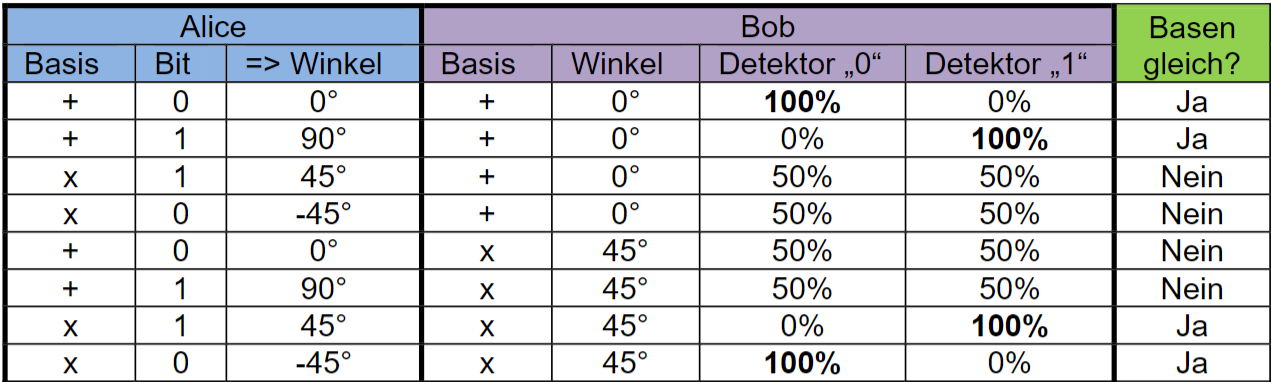
\includegraphics[width=0.65\textwidth]{content/grafik/Tabelle.png}
	\caption{Darstellung des gemessenen Bits in Abhängigkeit der Basis und gesendeten Bits. \cite{krypt}}
	\label{fig:Tabelle}
\end{figure}
Die genaue Basis wird gewählt, indem sich Alice und Bob nach eine gewissen Zeit über die Basen austauschen. Da, falls Alice und Bob die gleiche Basis hatten, auch das Bit übereinstimmt, kennen nun sowohl Sender als auf Empfänger den Schlüssel, welcher wie in \autoref{sec:Blabla} auf die ursprüngliche Nachricht addiert wird.
      
\section{Identifikation eines Abhörversuches}

Falls Lauscher Eve versucht, abzuhören, vermisst sie also das Licht, das von Alice kommt, und versucht, die identische Information an Bob weiterzuleiten. Dabei gibt es zwei Hauptmöglichkeiten. Wenn Eve die gleiche Basis wie Alice wählt, erhält sie das richtige Ergebnis und kann den Polarisationszustand korrekt an Bob weitergeben. Bob wählt nun zufällig seine Basis, was zu zwei möglichen Szenarien führt: Wenn Bob die gleiche Basis wie Alice wählt, erhält er den richtigen Polarisationszustand, ohne die Anwesenheit von Eve zu bemerken. Wählt Bob jedoch eine andere Basis, wird die Messung verworfen, da die Basen nicht übereinstimmen.

Wenn Eve hingegen die falsche Basis wählt, springt zufällig einer der Detektoren an. Auch hier gibt es zwei Möglichkeiten. Wenn Bob eine andere Basis als Alice wählt, wird die Messung beim Basenvergleich verworfen. Wenn Bob jedoch die gleiche Basis wie Alice wählt, führt dies zu einem Fehler. Dieser Fehler tritt auf, weil Eve die Basis falsch gewählt hat, was zu einer falschen Messung führt. In der Hälfte der Fälle wird Bob das richtige Bit erhalten, in der anderen Hälfte jedoch ein falsches Bit, das Eve übermittelt hat.
Auch hier ist es übersichtlicher eine Tabelle zur Darstellung zu verwenden (siehe \autoref{fig:Tabelle2}).
\begin{figure}[H]
	\centering
	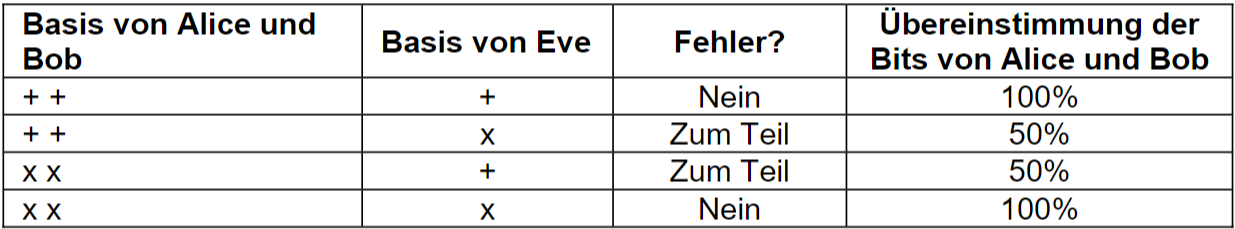
\includegraphics[width=0.65\textwidth]{content/grafik/Tabelle2.png}
	\caption{Fehler in Abhängigkeit der gewählten Basen des Abhörers \cite{krypt}}
	\label{fig:Tabelle2}
\end{figure}

\subsection{Analogei zum Quantenmechanischen Versuch}
Da es sich hierbei um einen Analogieversuch handelt, gilt es den Zusammenhang der beiden Betrachtungsweisen zu zeigen. Während im klassischen Fall ein Lichtpuls verwendet wird, werden beim der eigentlichen Quantenkryptografie Einzelphotonen verwendet.
\subsubsection{Zufall}
Wie bereits erwähnt, handelt es sich bei den Zufallszahlen, die durch einen klassischen Computer erzeugt werden um Pseudozufallszahlen, da diesen ein Algorithmus zugrunde liegt. 
In der QM ist das anders, hier gibt es "echte Zufälle". Der polarisierende Strahlteiler, der bei Bob und Eve verwendet wird, lässt im klassischen Fall einen Teil des Strahls transmittieren und den anderen reflektieren.
Bei der quantenmechanischen Betrachtung ist es jedoch vollkommen zufällig, ob das Photon bei $45\circ$-Rotation Transmittiert oder reflektiert wird. Im Analogieversuch wird es dadurch umgesetzt, dass elektronisch gesteuert wird, welcher Detektor "zufällig" anspringt.

\subsubsection{No-Cloning Theorem}
In der Quantenkryptografie, insbesondere im Quanten-Schlüsselverteilungsverfahren (z. B. BB84), wird der Sicherheitsmechanismus stark auf den Prinzipien der Quantenmechanik aufgebaut. Hier wird der Zustand des Lichts (z. B. Polarisation von Photonen) zur Übertragung von Schlüsselinformationen genutzt. Ein Lauscher, der versucht, den Schlüssel abzuhören, muss auf die Quantenbits zugreifen, die zwischen Alice und Bob übertragen werden.

Wenn ein Abhörer versucht, das quantenmechanische Signal zu messen und dabei zu klonen (um es weiterzugeben, ohne es zu verändern), verletzt er das No-Cloning-Theorem. Die Messung eines unbekannten Quantenzustandes verändert den Zustand. In der Praxis bedeutet dies, dass die Messung durch den Lauscher den Zustand des Signals verändert und diese Veränderung bei der späteren Überprüfung des Schlüssels erkennbar wird.

In Verfahren wie BB84 vergleichen Alice und Bob nach der Übertragung ihre Basiswahl und die gemessenen Werte. Wenn Eve den Abhörversuch unternimmt, wird sie die Quantenbits messen, was den Zustand des Signals beeinflusst. Da sie den unbekannten Zustand nicht perfekt klonen kann, wird ihre Messung Fehler in die Kommunikation einführen. Diese Fehler können durch Alice und Bob entdeckt werden, wenn sie die Basis und die erhaltenen Messwerte vergleichen. 
Wenn die Fehlerquote in den Schlüsseln zu hoch ist (normalerweise mehr als etwa 25\%), wissen Alice und Bob, dass ein Abhörer aktiv ist, da solche Fehler ohne Abhörversuch nicht auftreten würden.#

\subsubsection{Einzelphotonen vs. klassischem Licht}
Auch wenn es im Analogieversuch gerechtfertigt ist, einen Lichtpuls zu verwenden, würde das Verfahren bei quantenmechanischer Betrachtung unter der Verwendung eines Lichtpulses versagen. Grund hierfür ist, dass der gesamte Strahl die Information trägt und es somit möglich wäre einen kleinen Teil abzuzweigen,
während der größte Teil ungehindert an Bob geleitet wird.
Hier wird also deutlich, dass es sich nur um einen Analogieversuch und keineswegs um eine exakte Umsetzung der Quantenkryptografie handelt.

\subsection{Überführung in QM}
Nachdem die Analogie in den vorherigen Abschnitten begründet wurde, sollte es möglich sein, die Versuchsbeschreibung und theoretischen Grundlagen in eine für die QM adäquate Form zu bringen
Was oben bereits qualitativ beschrieben wurde, wird hier nochmal in der Dirac-Notation quantenmechanisch aufgearbeitet. 
 
Zu Beginn wird eine geeignete Notation gewählt, um Polarisationszustände zu beschreiben. Für diese Zwecke wird die Bra-Ket-Notation von Dirac verwendet. Die vier relevanten Polarisationszustände in diesem Experiment werden durch die Symbole
\[
| -45^\circ \rangle, |0^\circ \rangle, |45^\circ \rangle, |90^\circ \rangle
\]
dargestellt, wobei \(|0^\circ \rangle\) und \(|90^\circ \rangle\) die Basiszustände der sogenannten + Basis repräsentieren und \(|-45^\circ \rangle\) sowie \(|45^\circ \rangle\) die Zustände der x-Basis sind. Der Vorteil der Dirac-Notation liegt darin, dass die Zustände mathematisch behandelt werden können, ohne dass ein konkretes Koordinatensystem festgelegt werden muss.

Falls jedoch ein Koordinatensystem im \(xy\)-Raum spezifiziert wird, lassen sich die Zustände auch als Vektoren darstellen:
\[
|0^\circ \rangle = \begin{pmatrix} 0 \\ 1 \end{pmatrix}, \quad |90^\circ \rangle = \begin{pmatrix} 1 \\ 0 \end{pmatrix}
\]

Ein nützliches mathematisches Werkzeug ist das Skalarprodukt, das für zwei Zustände \(|a \rangle\) und \(|b \rangle\) folgendermaßen definiert wird:
\[
\langle 90^\circ | 0^\circ \rangle = \begin{pmatrix} 1 & 0 \end{pmatrix} \cdot \begin{pmatrix} 0 \\ 1 \end{pmatrix} = 0
\]
Das Betragsquadrat des Skalarprodukts stellt die Wahrscheinlichkeit dar, dass ein Photon mit Polarisation \(0^\circ\) durch einen Polarisator mit Orientierung \(90^\circ\) hindurchtritt. In diesem Fall ist diese Wahrscheinlichkeit null, was mit dem oben berechneten Ergebnis übereinstimmt.

Nun lässt sich jeder Zustand als Linearkombination der Basiszustände darstellen. Ein Beispiel ist der Zustand \(|45^\circ \rangle\), der sich wie folgt ausdrücken lässt:
\[
|45^\circ \rangle = \alpha \cdot |0^\circ \rangle + \beta \cdot |90^\circ \rangle
\]
Damit das Skalarprodukt normiert bleibt, muss gelten:
\[
\langle 45^\circ | 45^\circ \rangle = |\alpha|^2 + |\beta|^2 = 1
\]
Aufgrund der Symmetrie ergibt sich \(\alpha = \beta = \frac{1}{\sqrt{2}}\), und die Zustände werden entsprechend umgeschrieben:
\[
|45^\circ \rangle = \frac{1}{\sqrt{2}} |0^\circ \rangle + \frac{1}{\sqrt{2}} |90^\circ \rangle
\]
\[
|-45^\circ \rangle = \frac{1}{\sqrt{2}} |0^\circ \rangle - \frac{1}{\sqrt{2}} |90^\circ \rangle
\]
\[
|0^\circ \rangle = \frac{1}{\sqrt{2}} |45^\circ \rangle + \frac{1}{\sqrt{2}} |-45^\circ \rangle
\]
\[
|90^\circ \rangle = \frac{1}{\sqrt{2}} |45^\circ \rangle - \frac{1}{\sqrt{2}} |-45^\circ \rangle
\]

Mit diesen Formeln kann auch die Wahrscheinlichkeit berechnet werden, dass ein Photon mit Polarisation \(0^\circ\) durch einen \(45^\circ\)-Polarisator hindurchtritt:
\[
|\langle 45^\circ | 0^\circ \rangle |^2 = \left| \frac{1}{\sqrt{2}} \langle 45^\circ | 45^\circ \rangle \right|^2 = \frac{1}{2}
\]
Die Wahrscheinlichkeit, dass ein Photon mit \(0^\circ\) Polarisation einen Polarisator mit \(45^\circ\) besteht, beträgt somit 50%.

Im Experiment wird die Basis (entweder + oder x) vorgegeben, und es wird gemessen, welcher Detektor anspricht. Nun stellt sich die Frage, wie die Messung mathematisch beschrieben wird. Dafür werden die Operatoren \(\hat{M}_+\) und \(\hat{M}_\times\) eingeführt, die die Messung in der jeweiligen Basis beschreiben:
\[
\hat{M}_+ = |0^\circ \rangle \langle 0^\circ | - |90^\circ \rangle \langle 90^\circ |
\]
\[
\hat{M}_\times = |45^\circ \rangle \langle 45^\circ | - |-45^\circ \rangle \langle -45^\circ |
\]

Wenden wir nun den Operator für die gerade Basis auf die Zustände \(0^\circ\) und \(90^\circ\) an:
\[
\hat{M}_+ |0^\circ \rangle = |0^\circ \rangle \langle 0^\circ | 0^\circ \rangle - |90^\circ \rangle \langle 90^\circ | 0^\circ \rangle = |0^\circ \rangle
\]
\[
\hat{M}_+ |90^\circ \rangle = |0^\circ \rangle \langle 0^\circ | 90^\circ \rangle - |90^\circ \rangle \langle 90^\circ | 90^\circ \rangle = -|90^\circ \rangle
\]

Dies zeigt, dass bei einer Messung in der + Basis der Zustand entweder in der Form von \(|0^\circ \rangle\) oder \(|90^\circ \rangle\) wiedergegeben wird, je nachdem, welcher Zustand ursprünglich gemessen wurde.

Ein weiteres Beispiel sind die schräg polarisierten Zustände bei einer Messung in der schrägen Basis:
\[
\hat{M}_\times |45^\circ \rangle = |45^\circ \rangle \langle 45^\circ | 45^\circ \rangle - |-45^\circ \rangle \langle -45^\circ | 45^\circ \rangle = |45^\circ \rangle
\]
\[
\hat{M}_\times |-45^\circ \rangle = |45^\circ \rangle \langle 45^\circ | -45^\circ \rangle - |-45^\circ \rangle \langle -45^\circ | -45^\circ \rangle = -|-45^\circ \rangle
\]

Nun wird beschrieben, wie sich der Zustand des Photons bei der Messung verändert. Im folgenden Abschnitt werden die Messungen und Zustände für Alice, Bob und Eve mithilfe der zuvor erarbeiteten mathematischen Grundlagen formuliert. Zu Beginn wird eine Tabelle ohne Eve (siehe \autoref{fig:Tabelle3}) gezeigt, später dann mit ihr (siehe \autoref{fig:Tabelle4}).


\begin{figure}[H]
	\centering
	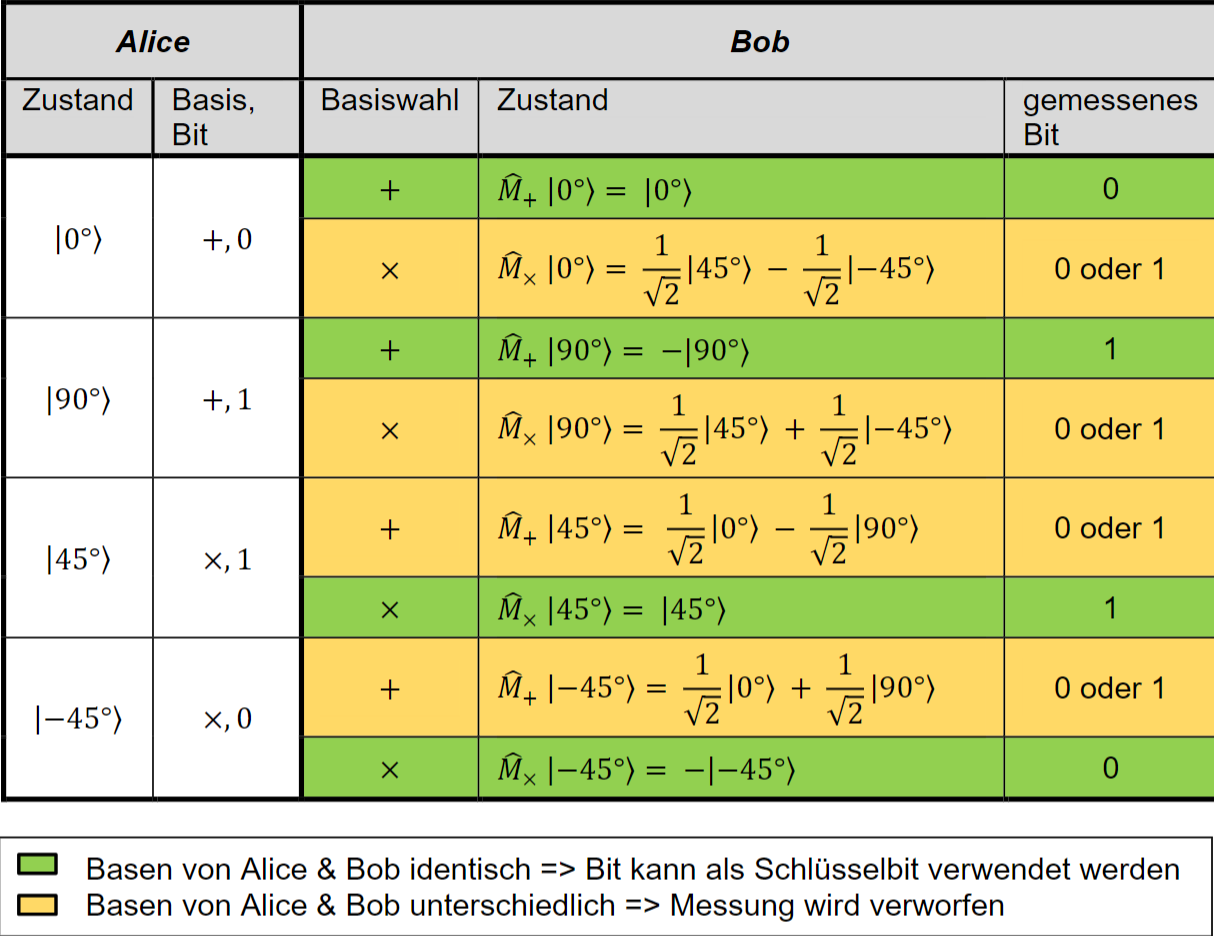
\includegraphics[width=0.65\textwidth]{content/grafik/Tabelle3.png}
	\caption{Tabellarische Darstellung der Zustände in Abhängigkeit der Basen ohne Abhörversuch\cite{krypt}}
	\label{fig:Tabelle3}
\end{figure}

\begin{figure}[H]
	\centering
	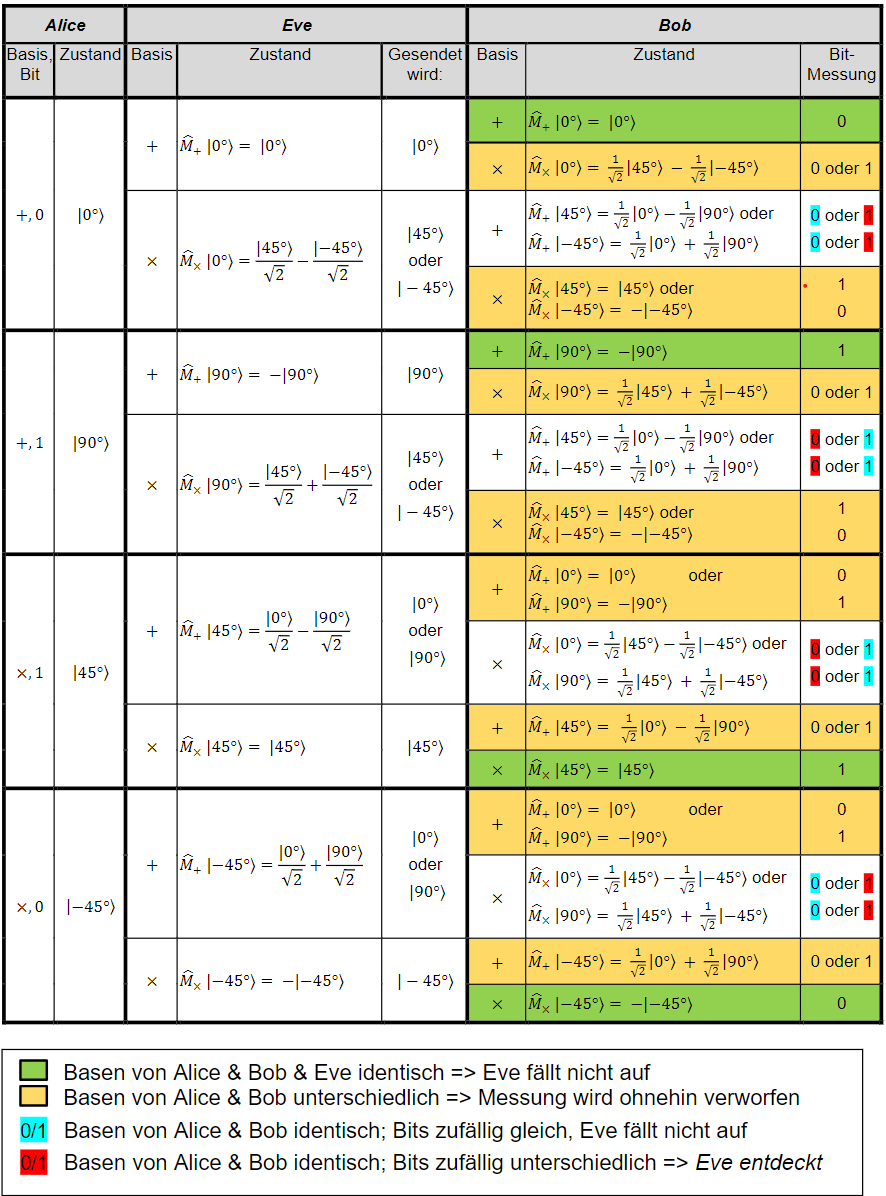
\includegraphics[width=0.65\textwidth]{content/grafik/Tabelle4.png}
	\caption{Tabellarische Darstellung der Zustände in Abhängigkeit der Basen mit Abhörversuch\cite{krypt}}
	\label{fig:Tabelle3}
\end{figure}